% !TEX encoding = UTF-8 Unicode
% !TEX root = FinalProject.tex

%%%  This is the main driver file.   It is mostly a list of file includes.   Read through and edit as needed.

\documentclass[table]{book}


\usepackage[width=6.5in, height=9.0in, top=1.0in, papersize={8.5in,11in}]{geometry}
\usepackage[pdftex]{graphicx}
\DeclareGraphicsExtensions{.pdf,.png,.jpg}
%\usepackage{draftwatermark}
\usepackage{amsmath}
\usepackage{amsthm}
\usepackage{amssymb}
%\usepackage{txfonts}
\usepackage{textcomp}
%\usepackage{amsthm}
%\usepackage{array}
%\usepackage{datetime}
%\usepackage{anyfontsize}
\usepackage{listings}
\usepackage{t1enc}
\usepackage[section,subsection]{extraplaceins}   %%%  \FloatBarrier
\usepackage[all]{xy}
\usepackage{fancyhdr}
\usepackage{hyperref}
\usepackage{verbatim}
\usepackage{algorithm}
\usepackage{algorithmic}
\usepackage{makeidx}
\usepackage{multicol}
\usepackage{multirow}
\usepackage{color}
\usepackage{rotating}
\usepackage{wrapfig}
\usepackage{tikz}
\usetikzlibrary{shapes.geometric, arrows}
%\usepackage{tabularx}
\usepackage{xcolor}
%\usepackage{framed}
\usepackage{xspace}
\usepackage{listings}
\lstset{language=python,frame=ltrb,framesep=5pt,basicstyle=\normalsize,
 keywordstyle=\ttfamily\color{DarkRed},
%morecomment=[n][\textbf]{In\ [}{]\:},
%morecomment=[n][\textbf]{Out\ [}{]\:},
morecomment=[s][\color{blue}]{In\ [}{]\:},
morecomment=[s][\color{red}]{Out[}{]\:},
identifierstyle=\ttfamily\color{DarkBlue}\bfseries,
commentstyle=\color{OliveGreen},
stringstyle=\ttfamily,
showstringspaces=false,tabsize = 3}

\lstdefinelanguage{shell} {
commentstyle = \color{black},
keywordstyle = \color{black},
stringstyle = \color{black},
identifierstyle = \color{black},
morecomment=[s][\color{blue}]{In\ [}{]\:},
morecomment=[s][\color{red}]{Out[}{]\:},
 }

\newtheorem{thrm}{Theorem}
\newtheorem{lem}[thrm]{Lemma}
\newtheorem{cor}[thrm]{Corollary}
\newtheorem{rem}[thrm]{Remark}
\newtheorem{defn}[thrm]{Definition}
\newtheorem{exmpl}[thrm]{Example}

% this gives a little box for the end of a proof:
%
\def\endthrmbox{$\sqsubset \!\!\!\! \sqsupset$}

\newcommand{\dis}{\displaystyle}
 \def      \RR             {{\mathbb R}} 
        \def      \NN             {{\Bbb N}} 
        \def      \QQ             {{\Bbb Q}} 
        \def      \CC             {{\Bbb C}} 
        \def      \ZZ             {{\Bbb Z}} 
 
 
        \def       \a              {{\alpha}} 
        \def       \b              {{\beta}} 
        \def       \d              {{\delta}} 
        \def       \D              {{\Delta}} 
        \def         \e              {{\varepsilon}} 
        \def         \g              {{\gamma}} 
        \def         \G              {{\Gamma}} 
        \def       \l              {{\lambda}} 
        \def       \L              {{\Lambda}} 
        \def        \m               {{\mu}} 
        \def         \n              {{\nabla}} 
        \def       \var          {{\varphi}} 
        \def         \s              {{\sigma}} 
        \def       \Sig          {{\Sigma}} 
        \def       \Om          {{\Omega}} 
 
        \def       \t              {{\tau}} 
        \def         \th             {{\theta}} 
        \def       \O              {{\Omega}} 
        \def       \o              {{\omega}} 
        \def         \z              {{\zeta}} 
       \def        \P             {{\Phi}} 
       \def        \p             {{\phi}} 
        %Other macros 
 
        \def       \iy              {{\infty}} 
        \def         \pa             {{\partial}} 
        \def         \div           {{\rm div}} 
         \def       \na            {{\nabla}} 
 



\newcommand{\pythonlogo}{
\\[-2mm] \begin{picture}(0,0)
\put(-40,-40){\includegraphics[scale=0.25]{./Figures/pythonlogo.png}}
\end{picture}
}

\newcommand{\clogo}{
\\[-2mm] \begin{picture}(0,0)
\put(-30,-30){\includegraphics[scale=0.2]{./Figures/clogo.png}}
\end{picture}
}

\newcommand{\roslogo}{
\\[-2mm] 
\begin{picture}(0,0)
\put(-30,-30){\includegraphics[scale=0.2]{./Figures/roslogo.png}}
\end{picture}
}


\tikzstyle{master} = [rectangle, draw, text width=6em, text centered, minimum
height=3em]
\tikzstyle{node} = [rectangle, draw, text width=6em, text centered, rounded
corners, minimum height=3em]

\newtheorem{summary}{Summary:}
\newtheorem{example}{Example:}[section]

\definecolor{OliveGreen}{cmyk}{0.64,0,0.95,0.40}
\definecolor{DarkBlue}{cmyk}{0.76,0.76,0,0.20}
\definecolor{DarkRed}{cmyk}{0,1,1,0.45}


\def      \RR             {{\mathbb R}} 
\def      \DS            {\displaystyle} 

\setlength{\oddsidemargin}{0mm} 
\setlength{\evensidemargin}{0mm} 

%\SetWatermarkLightness{0.975}
%\SetWatermarkScale{6}
%\SetWatermarkText{\includegraphics{test.png}}

\pagestyle{fancy}
\renewcommand{\chaptermark}[1]{\markboth{#1}{}}
\renewcommand{\sectionmark}[1]{\markright{\thesection\ #1}}
\fancyhf{}
\fancyhead[LE,RO]{\bfseries\thepage}
\fancyhead[LO]{\bfseries\rightmark}
\fancyhead[RE]{\bfseries\leftmark}
\renewcommand{\headrulewidth}{0.5pt}
\renewcommand{\footrulewidth}{0pt}
\addtolength{\headheight}{0.5pt}
\setlength{\footskip}{0in}
\renewcommand{\footruleskip}{0pt}
\fancypagestyle{plain}{%
\fancyhead{}
\renewcommand{\headrulewidth}{0pt}
}


\definecolor{color02}{rgb}{0.18,0.35,0.59}
\definecolor{color03}{rgb}{0.44,0.59,0.82}
\definecolor{color06}{rgb}{0.35,0.35,0.35}


\definecolor{MSBlue}{rgb}{.204,.353,.541}
\definecolor{MSLightBlue}{rgb}{.31,.506,.741}
\definecolor{MSBlue1}{rgb}{0.18,0.35,0.59}
\definecolor{MSBlue2}{rgb}{0.44,0.59,0.82}
\definecolor{MSBlue3}{rgb}{0.35,0.35,0.35}

\usepackage{titlesec}
\titleformat{\chapter}[display]
%{\normalfont\bfseries\color{MSBlue1}}    %\normalfont\bfseries\filcenter}
{\normalfont\bfseries}    %\normalfont\bfseries\filcenter}
{\LARGE\thechapter}
{1ex}
{\titlerule[2pt]
\vspace{2ex}%
\LARGE}
[\vspace{1ex}%
{\titlerule[2pt]}]



\date{\today}

 % This sets the format.

% Add your title page contents here 
\title{{ \rule{\linewidth}{0.5mm}}\\[2mm] {\huge \bfseries  Project Title }\\[-1mm] {\rule{\linewidth}{0.5mm}} \\  \vfill
{\LARGE \bfseries  Natural Computing Final Project }\vfill}
\author{Derek Stotz \and  Christopher Smith  }
\date{\today}


\begin{document}

\frontmatter

% Comment out items you don't need

\addcontentsline{toc}{chapter}{Title}
\maketitle
\tableofcontents
\addcontentsline{toc}{chapter}{Contents}
\listoffigures
\addcontentsline{toc}{chapter}{List of Figures}
\listoftables
\addcontentsline{toc}{chapter}{List of Tables}
\listofalgorithms
\addcontentsline{toc}{chapter}{List of Algorithms}

\chapter{Document Preparation and Updates}
% !TEX root = FinalProject.tex



Current Version [X.X.X]
\vspace*{5mm}

{\color{MSBlue3}
\noindent
\textit{Prepared By:}\\
\textit{Team Member \#1}\\
\textit{Team Member \#2}\\
\textit{Team Member \#3}
}

\vfill
\noindent
{\color{color02} \textit{\textbf{Revision History}}}\\
\begin{tabular}{|>{\raggedright}p{1.5cm}|>{\raggedright}p{3cm}|>{\raggedright}p{1.5cm}|>{\raggedright}p{9cm}|}
\hline
\textit{\textbf{Date}} &  \textit{\textbf{Author}} & \textit{\textbf{Version}} & \textit{\textbf{Comments}}\tabularnewline
\hline
 \textit{\textbf{2/2/15}} & \textit{Team Member \#1} & \textit{1.0.0} & \textit{Initial version}\tabularnewline
\hline
\textit{\textbf{3/4/15}} & \textit{Team Member \#3} & \textit{1.1.0} & \textit{Edited version}\tabularnewline
\hline
 &  &  & \tabularnewline
 \hline
 &  &  & \tabularnewline
\hline
 &  &  & \tabularnewline
\hline
 &  &  & \tabularnewline
\hline
 &  &  & \tabularnewline
\hline
\end{tabular}
\vfill


 
 % Core content to follow ...
 
\mainmatter

%%  Add to the following chapters
% you may also need additional chapters ...

% !TEX root = FinalProject.tex

\chapter{Introduction}

Introduce your project. 

\section{Overview}
Provide a description.  

\section{Background}

Literature review here.  Background work.   
% !TEX root = FinalProject.tex

\chapter{Problem}

The board game Puerto Rico is a beloved Euro game of critical acclaim and widespread popularity.  It involves indirect player interaction through the building of a Caribbean island colony, where the players compete for money and victory points via exports and sales of their cash crops. Puerto Rico is simple to learn but hard to master because of all the decision making the player has to do throughout the game.  This means that the actions, while simple to represent, are very difficult to pick in different situations... making the choices of actions perfect for one of the techniques discussed in class.  Our goal is to develop an AI capable of playing puerto rico with a human with 3 players. 
 




% !TEX root = FinalProject.tex

\chapter{Implementation}

We implemented our simulation of Puerto Rico using python3 and a variety of standard libraries, such as OS, math, sys, and random.  Non-standard libraries include Pickle and Enum.  Pickle was used for serialization while Enum was used for some more readable type information... enum was included in the project for Opp lab issue reasons, but pickle might still need to be installed on the user's computer in order to run this project. \\

The GA is based on one written for Homework 2 of the course, while the ANN is a translation of Dr. Pyeatt's code from C++.  Future versions of the code may use Numpy to speed things up, or perhaps implement Cython for improved performace.  The GA is meant to be run ahead of time, and the main game runs more than fast enough for end user purposes.
% !TEX root = FinalProject.tex

\section{The Game }

\section{Evolutionary Algorithm}
The evolutionary algorithm \ref{alg1} for this program starts off randomly creating a population of two thousand and then evaluating two thousand generations. The population is first initialized and evaluated. The best individual is kept and stored. All individuals equal in fitness are also kept between the generations. After the best fitness is found the all the bad fitness individuals are selected for recombination based on the the best individuals that population. A new generation is created based on the best fitness individuals and the ones recombined based off of their weights. The genetic algorithm takes care of selecting weights to recombine as well as the mutation rate for individual offspring, while the tournament selection handles the evaluation of an individual during the game based on how many times they win and become runner up.

\begin{algorithm} [tbh]                     % enter the algorithm environment
\caption{Evolve ANNs}          % give the algorithm a caption
\label{alg1}                           % and a label for \ref{} commands later in the document
\begin{algorithmic}                    % enter the algorithmic environment
    \STATE initialize population
    \STATE evaluate population
    \FOR{ i in range( number\_of\_generations ) }
    	\STATE get top fitness
    	\FOR{ p in population }
    		\FOR{k in range( 0 , keep ranks)}
    			\IF{ keep[k] < p.fitness and not (p.fitness in keep) }
    				\STATE keep[k] = p.fitness
    			\ENDIF
    		\ENDFOR
    	\ENDFOR
    \ENDFOR
\end{algorithmic}
\end{algorithm}

\subsection{Genetic Algorithm}
\subsection{Tournament Selection}

\section{The ANNs }
The Artificial Neural Network used for this project was a modified ANN from Dr. Pyeatte's code. We converted his ANN to python and removed the back-propagation function and saving and loading from files. We added a mutation function and a recombination function. The mutation function takes the number of weights that are to be mutated then randomly chooses that number of weights and randomly assigns them a value. The recombination function takes to lists of weights as arguments and gives a 50-50 chance of choosing a weight from one or the other to create its own weights.

See Figure~\ref{systemdiagram}.  This is an example of a building phase ANN. The whole game board is given as inputs to the neural network. The number of colonists, each building and plantation type, number of each resource, victory points, and the amount of dabloons they have are all given under the player inputs. Player1 inputs used to save space in the figure. All of this information fed through the hidden layers and then outputs in the building phase are ranked. The higher the output the better the option is. The player will start with the best ranked option and try to do it. If it doesn't have enough dabloons to buy it the next option is chosen and repeats until something is bought or buy nothing is chosen.
\begin{figure}[tbh]
\begin{center}
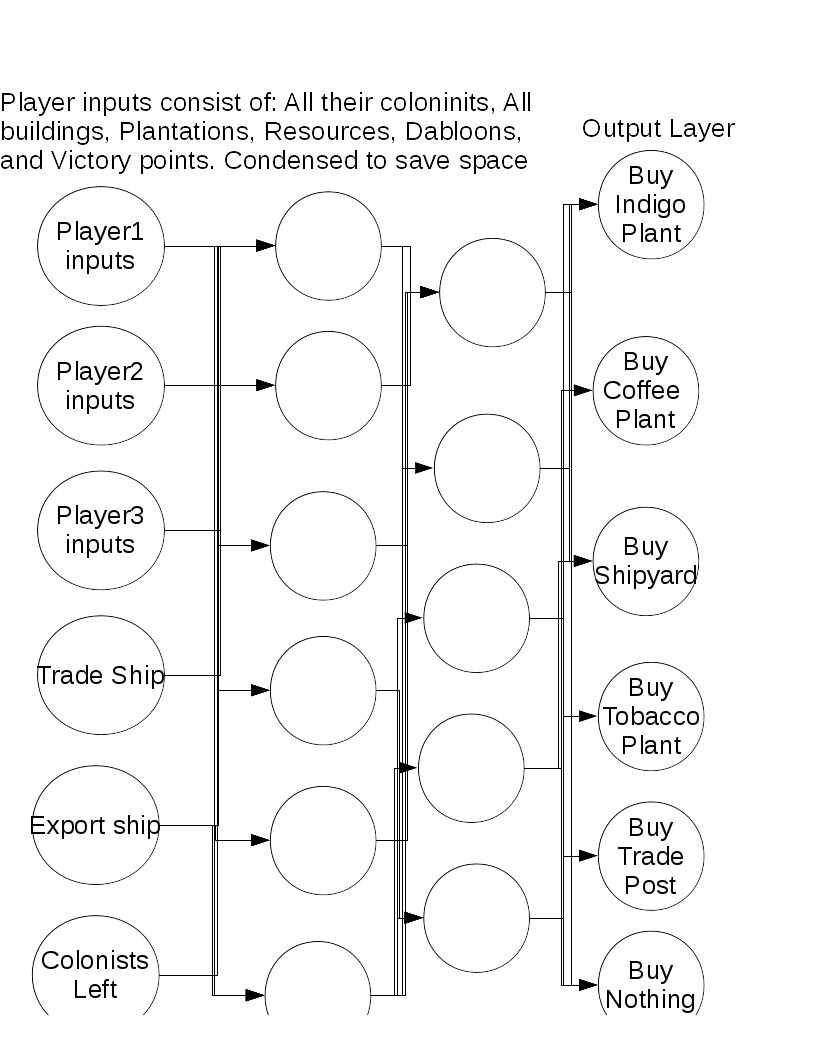
\includegraphics[width=0.75\textwidth]{./images/Example_ANN.png}
\end{center}
\caption{A example of a building phase ANN \label{systemdiagram}}
\end{figure}

\begin{algorithm} [tbh]                     % enter the algorithm environment
\caption{Calculate $y = x^n$}          % give the algorithm a caption
\label{alg1}                           % and a label for \ref{} commands later in the document
\begin{algorithmic}                    % enter the algorithmic environment
    \REQUIRE $n \geq 0 \vee x \neq 0$
    \ENSURE $y = x^n$
    \STATE $y \Leftarrow 1$
    \IF{$n < 0$}
        \STATE $X \Leftarrow 1 / x$
        \STATE $N \Leftarrow -n$
    \ELSE
        \STATE $X \Leftarrow x$
        \STATE $N \Leftarrow n$
    \ENDIF
    \WHILE{$N \neq 0$}
        \IF{$N$ is even}
            \STATE $X \Leftarrow X \times X$
            \STATE $N \Leftarrow N / 2$
        \ELSE[$N$ is odd]
            \STATE $y \Leftarrow y \times X$
            \STATE $N \Leftarrow N - 1$
        \ENDIF
    \ENDWHILE
\end{algorithmic}
\end{algorithm}

\section{Training the ANNs }

% !TEX root = FinalProject.tex
\section{The Main }


\chapter{Issues}
\section{Issues }

% !TEX root = FinalProject.tex

\section{Results}

Our delivered project was very fun and interesting.  While we did not specifically deliver what we set out to do, as the evolution of AIs was more difficult than we had initially hoped, Derek would love to continue exploring it over the summer, expanding its functionality and overcoming its limitations.


\subsection{Expectations}

Initially, we planned on evolving AIs which would have some level of recognizable decision making skills.  At the very least, we wanted to evolve garbage AIs with little to no decision making, demonstrating the ability to apply EA concepts to our neural network.

\subsection{Issues}

We initially split our project into two parts - Derek would adapt the GA code into our desired evolutionary algorithm and write the game simulation, while Chris would handle the neural network.  It seemed like a decent split of the work.  By the time the presentation was presented, we had completed the neural network and evolutionary algorithm and tested them by evolving neural nets which could add two two-bit numbers without calculating anything.  In addition, Derek had completed writing all of the game simulation but half of the phases and the interface to the nerual nets - the project seemed nearly complete. \\

After dozens of straight hours of work, debugging, and code refactoring the following week, Derek realized how much he had gravely underestimated the work load he had allocated to himself.  In the end, however, he refused to give up even when staring into the cruel face of his own stupidity, and managed to finish the AI.\\

The biggest issue with evolving the AIs, unfortunately, was discovered right at the end of the debugging process.  Even when functioning 100 percent, the AIs tended to not change their role selection sufficiently enough to keep the game advancing towards completion.  It required an AI who occationally picked the mayor phase to lead the game to the end.  Too often the AIs would get stuck in a loop where they all selected some combination of roles which would not affect the game state, ensuring the exact same selection next time.  While this could be temporarily solved with a diff function which killed the game when no change in game state was discovered, the behavioral flaw was so prevalent that it is clear that it would take a major overhaul of the evolutionary sysem to overcome the limitation.

\subsection{Results}

When running a game of Puerto Rico with 1 AI, the decisions it makes seem generally random - because they are.  We were unable to actually evolve the AIs, so the result is a very stupid simulation of another player, which is fairly amusing but not at all challenging to defeat.  It is clear that it could become something very impressive, but at the moment is more of a proof of concept. \\

The AIs are a definite success, as they are flexible, fast, and can develop decision-making abilities when evolved, as our trial with the adders mentioned earlier proved.  Unfortunately, we have yet to see them in action as they were intended. \\

The evolutionary algorithm was a moderate success - it does what it was designed to do, and does it with quite a bit of efficiency and tunability.  Unfortunately, it doesn't really work, and requires the most rewriting by far out of any of the files in the project. \\

The game simulation was a roaring success.  The code is monstrous and ugly and labywrinthine and machiavellian, but beautiful in its own way.  It could use some rewriting, and probably a good ditching of the Enum library for some straight classes and constants, but it does its job very well and simulates a game of Puerto Rico down to the last doubloon.  There may be some bugs left in relation to its janky interface with the AI, but overall it's pretty smooth.

\subsection{Extensibility}

Derek would love to explore this in the future, and probably will dedicate some time to it this summer.  Firstly, an EA should be developed which can reliably improve the performance of the AIs in the population, even if it takes an age of this world to do so.  The inifinite loops are unacceptable.  Secondly, the game should be generalized for more than 3 players and the game state should take into account more things, including what's on the boards of other players.  While this would exponentially increase the difficulty of evolving the AIs, it would allow for some more sophisticated strategies to emerge.  Lastly, other projects - perhaps even thesis-grade ones - could be spun off from this one, like writing simulations for other board games which utilize the same evolutionary and AI system, building a robot to play the board games while using the AI and simluation as a brain, or even a system to not only learn good strategies but even the rules of the board game itself, generalizing the system for any and all board gamess imaginable.  That last one may be a moon shot, but it would be pretty awesome.

\subsection{Conclusion}

We are very happy with how the program turned out, and find it to be a fun application of Natural Computing principles.  It is a definite example of how the fundamental elements of this course can be applied to solve problems and creates something new with fascinating emergent behaviors.  Unfortunately, the production was botched and ended up taking too long.  We apologize for any inconvenice it may have caused, but we wanted to make sure that the project which we handed in was a complete one, and not a half-baked one with less tardiness.

%%%  Done with chapters
% Bib stuff

\bibliographystyle{plain}
\bibliography{refs.bib}
\addcontentsline{toc}{chapter}{Bibliography}



% In our style file, appendices are numbered with capital letters
\appendix

\chapter{Supporting Materials}

This document will contain several appendices used as a way to separate out major 
component details, logic details, or tables of information.  Use of this structure 
will help keep the document clean, readable, and organized. 



\chapter{Code}
Insert code here.   You can use the listing environment or use doxygen.



% chapters in backmatter don't have numbers, but they appear in the
% table of contents, and are numbered BM-X where X is the page number
% relative to where the backmatter begins.
\backmatter


%%  The author of LaTeX provided all of us with a sample document.  Here it is ...
\chapter{\LaTeX\ Example}
% !TEX root = FinalProject.tex


\LaTeX\xspace sample file:  

\section{Introduction}
This is a sample input file.  Comparing it with the output it
generates can show you how to produce a simple document of
your own.

\section{Ordinary Text}  % Produces section heading.  Lower-level
                                    % sections are begun with similar 
                                    % \subsection and \subsubsection commands.

The ends  of words and sentences are marked 
  by   spaces. It  doesn't matter how many 
spaces    you type; one is as good as 100.  The
end of   a line counts as a space.

One   or more   blank lines denote the  end 
of  a paragraph.  

Since any number of consecutive spaces are treated like a single
one, the formatting of the input file makes no difference to
      \TeX,         % The \TeX command generates the TeX logo.
but it makes a difference to you.  
When you use
      \LaTeX,       % The \LaTeX command generates the LaTeX logo.
making your input file as easy to read as possible
will be a great help as you write your document and when you
change it.  This sample file shows how you can add comments to
your own input file.

Because printing is different from typewriting, there are a 
number of things that you have to do differently when preparing 
an input file than if you were just typing the document directly.  
Quotation marks like 
       ``this'' 
have to be handled specially, as do quotes within quotes: 
       ``\,`this'                  % \, separates the double and single quote.
        is what I just 
        wrote, not  `that'\,''.  

Dashes come in three sizes: an 
       intra-word 
dash, a medium dash for number ranges like 
       1--2, 
and a punctuation 
       dash---like 
this.

A sentence-ending space should be larger than the space between words
within a sentence.  You sometimes have to type special commands in
conjunction with punctuation characters to get this right, as in the
following sentence.
       Gnats, gnus, etc.\    % `\ ' makes an inter-word space.
       all begin with G\@.   % \@ marks end-of-sentence punctuation.
You should check the spaces after periods when reading your output to
make sure you haven't forgotten any special cases.
Generating an ellipsis 
       \ldots\    % `\ ' needed because TeX ignores spaces after 
                  % command names like \ldots made from \ + letters.
                  %
                  % Note how a `%' character causes TeX to ignore the 
                  % end of the input line, so these blank lines do not
                  % start a new paragraph.
with the right spacing around the periods 
requires a special  command.  

\TeX\ interprets some common characters as commands, so you must type
special commands to generate them.  These characters include the
following: 
       \$ \& \% \# \{ and \}.

In printing, text is emphasized by using an
       {\em italic\/}  % The \/ command produces the tiny extra space that
                       % should be added between a slanted and a following
                       % unslanted letter.
type style.  

\begin{em}
   A long segment of text can also be emphasized in this way.  Text within
   such a segment given additional emphasis 
          with\/ {\em Roman} 
   type.  Italic type loses its ability to emphasize and become simply
   distracting when used excessively.  
\end{em}

It is sometimes necessary to prevent \TeX\ from breaking a line where
it might otherwise do so.  This may be at a space, as between the
``Mr.'' and ``Jones'' in
       ``Mr.~Jones'',        % ~ produces an unbreakable interword space.
or within a word---especially when the word is a symbol like
       \mbox{\em itemnum\/} 
that makes little sense when hyphenated across 
       lines.

Footnotes\footnote{This is an example of a footnote.}
pose no problem.

\TeX\ is good at typesetting mathematical formulas like
       \( x-3y = 7 \) 
or
       \( a_{1} > x^{2n} / y^{2n} > x' \).
Remember that a letter like
       $x$        % $ ... $  and  \( ... \)  are equivalent
is a formula when it denotes a mathematical symbol, and should
be treated as one.

\section{Displayed Text}

Text is displayed by indenting it from the left margin.
Quotations are commonly displayed.  There are short quotations
\begin{quote}
   This is a short a quotation.  It consists of a 
   single paragraph of text.  There is no paragraph
   indentation.
\end{quote}
and longer ones.
\begin{quotation}
   This is a longer quotation.  It consists of two paragraphs
   of text.  The beginning of each paragraph is indicated
   by an extra indentation.

   This is the second paragraph of the quotation.  It is just
   as dull as the first paragraph.
\end{quotation}
Another frequently-displayed structure is a list.
The following is an example of an {\em itemized} list.
\begin{itemize}
   \item  This is the first item of an itemized list.  Each item 
          in the list is marked with a ``tick''.  The document
          style determines what kind of tick mark is used.

   \item  This is the second item of the list.  It contains another
          list nested inside it.  The inner list is an {\em enumerated}
          list.
          \begin{enumerate}
              \item This is the first item of an enumerated list that
                    is nested within the itemized list.

              \item This is the second item of the inner list.  \LaTeX\
                    allows you to nest lists deeper than you really should.
          \end{enumerate}
          This is the rest of the second item of the outer list.  It
          is no more interesting than any other part of the item.
   \item  This is the third item of the list.
\end{itemize}
You can even display poetry.
\begin{verse}
   There is an environment for verse \\    % The \\ command separates lines
   Whose features some poets will curse.   % within a stanza.

                           % One or more blank lines separate stanzas.

   For instead of making\\
   Them do {\em all\/} line breaking, \\
   It allows them to put too many words on a line when they'd 
   rather be forced to be terse.
\end{verse}

Mathematical formulas may also be displayed.  A displayed formula is
one-line long; multi-line formulas require special formatting
instructions.
   \[  x' + y^{2} = z_{i}^{2}\]
Don't start a paragraph with a displayed equation, nor make
one a paragraph by itself.

\section{Build process}

To build \LaTeX\ documents you need the latex program.  It is free and available on all operating systems.   Download and install.  Many of us use the TexLive distribution and are very happy with it.    You can use a editor and command line or use an IDE.  To build this document via command line:

\begin{verbatim}
alta>  pdflatex SystemTemplate
\end{verbatim}
If you change the bib entries, then you need to update the bib files:
\begin{verbatim}
alta>  pdflatex SystemTemplate
alta>  bibtex SystemTemplate
alta>  pdflatex SystemTemplate
alta>  pdflatex SystemTemplate
\end{verbatim}

The template files provided also contain a Makefile, which will
make things much easier.  

\section*{Acknowledgment}
Thanks to Leslie Lamport.  






\end{document}
